\documentclass{aiaa-tc}

%\usepackage[margin=1.0in]{geometry}
\usepackage{fullpage}
\usepackage{graphicx}
\usepackage{bm} %required for bold in math mode for greek symbols
\usepackage{amsmath} %for bmatrix
\usepackage{amsfonts} %for math script font
\usepackage{url} %for website citations

\usepackage[space]{grffile} %for filepaths with spaces

%define degree symbol:
\newcommand{\degree}{\ensuremath{^\circ}}

\newcommand{\fr}[1]{$#1^+$} %command to write a reference frame
\newcommand{\br}[2]{[#1]_{#2}} %bracket operator with subscript
\newcommand{\tvect}[3]{\begin{bmatrix}#1\\#2\\#3\end{bmatrix}}% 3 x 1 vector
\newcommand{\tvecth}[3]{\begin{bmatrix}#1&#2&#3\end{bmatrix}}% 1 x 3 vector
\newcommand{\B}[1]{\textbf{#1}} %bold for regular vectors
\newcommand{\U}[1]{\hat{\textbf{#1}}} %hats and bold for unit vectors
\newcommand{\BG}[1]{{\bm #1}}           % for vectors using greek letters
\newcommand{\ddt}[1]{\frac{d#1}{dt}} %for time derivatives
\newcommand{\kron}{\otimes} %redefines \kron to produce kronecker product symbol, for convenience

\title{System identification for Parrot AR.drone}
\author{Tim Woodbury}

\let\endtitlepage\relax %surpress line break after title page

% outline:
% intro
%	What is the goal
%	Why is it relevant
%	How is it performed
%	How are results generated and analyzed
% Background
%	Dynamic model
% 	Identification algorithms
%		list, no theory
% Identified candidate model and performance 
%	model
%	MSQ table
%	Sample plots
%


\begin{document}

\maketitle

A key element of the estimation scheme planned for implementation in the quadrotor lab is inclusion of vehicle drag coefficients as linear function of body-axis 1 and 2 velocity components. Inclusion of these terms is expected to enable high-fidelity attitude estimation than would otherwise be possible. Using the Optitrack motion capture system, the rigid body position and attitude histories of a quadrotor vehicle can be captured to a high degree of accuracy, enabling system identification from flight data with relatively little data processing. Linear system identification methods are then used to identify models of the velocity states as functions of the vehicle attitude as effective controls. Model selection is performed using mean squared error as the performance metric.

\section{Background}

This section presents the linearized dynamic model assumed and briefly describes the identification schemes used.

\subsection{Dynamic model}

The exact velocity-level kinematics of the quadrotor can be derived easily. A body-fixed reference frame is established as a 3-2-1 Euler angle rotation from a north-east-down inertial reference frame. From a trim state of zero velocity and zero pitch and roll, the linearized equation for body-axis velocities $u$ and $v$ in terms of bank and pitch angles $\phi$ and $\theta$ is:

\begin{equation}
\begin{bmatrix}
\dot{u} \\
\dot{v}
\end{bmatrix} = \begin{bmatrix}
c_D & 0 \\ 0 & c_D
\end{bmatrix}
\begin{bmatrix}
u \\
v
\end{bmatrix}
+
\begin{bmatrix}
-g & 0 \\
0 & g
\end{bmatrix}
\begin{bmatrix}
\theta \\
\phi
\end{bmatrix}
\end{equation}

Here, $c_D$ is the unknown drag coefficient of interest and $g$ is gravitational acceleration.

\subsection{System identification}

Both Observer/Kalman filter identification (OKID) and a direct discrete-time least-squares model are fit to the data. Readers desiring a detailed look at OKID should be directed to Jer-Nan Juang's ``Applied System Identification.'' As a check against OKID, a linear discrete-time model of the form $x_{k+1} = Ax_k + Bu_k$ is fit in a least-squares sense to the data.

Data were segmented manually such that each segment began near a trim state and avoided bad tracking from the Optitrack system. Two linear models were fit to each segment, one using OKID and one using the least-squares model.

\section{Results}

\subsection{Identified model}

The identified continuous-time system has $c_D = -.13$ s${}^{-1}$. This is achieved by averaging the coefficients for the $u$ and $v$ terms. Results are presented in terms of the mean squared error (MSE), defined in terms of $n$ measurements (assumed truth) $\tilde{y}_i$ and model predictions $\hat{y}_i$:

\begin{equation}
MSE = \frac{1}{n} \sum_{i=1}^n (\tilde{y}_i-\hat{y}_i)^2
\end{equation}

MSE is computed separately for $u$ and $v$ terms. Data from two flight days are used for identification and validation. Predicted outputs were generated by feeding the attitude histories into the identified model, beginning the from the same initial state as the flight data, and evaluating the development of the system in time. It was assumed that the ``best'' model should have a consistently low MSE for any given segment of data. Three segments are identified on day 1, and four on day 2. The MSE of the identified model with respect to each axis is given in Table \ref{tab:mses}. This model was selected because it achieved MSEs of the order of $0.01$ for both axes on more segments than the other identified models did, which is thought to indicate better consistency overall.

\begin{table}[tb!]
\centering
\begin{tabular}{c|c|c|c}
Day & Segment & $MSE_u$ & $MSE_v$ \\
1 & 1 & 0.051 & 0.012 \\
1 & 2 & 0.045  &   0.016\\
1 & 3 & 0.052  &   0.028\\
2 & 1 & 0.099  &    0.14\\
2 & 2 & 0.11  &     0.14\\
2 & 3 & 0.064 &   0.14\\
2 & 4 & 0.023  &   0.12\\
\end{tabular}
\caption{MSEs for the identified model against difference flight data.}
\label{tab:mses}
\end{table}

To qualitatively evaluate the model, predicted and measured outputs are given in Figs. \ref{fig:day1mse}-\ref{fig:day2mse}.

\begin{figure}[tb!]
\centering
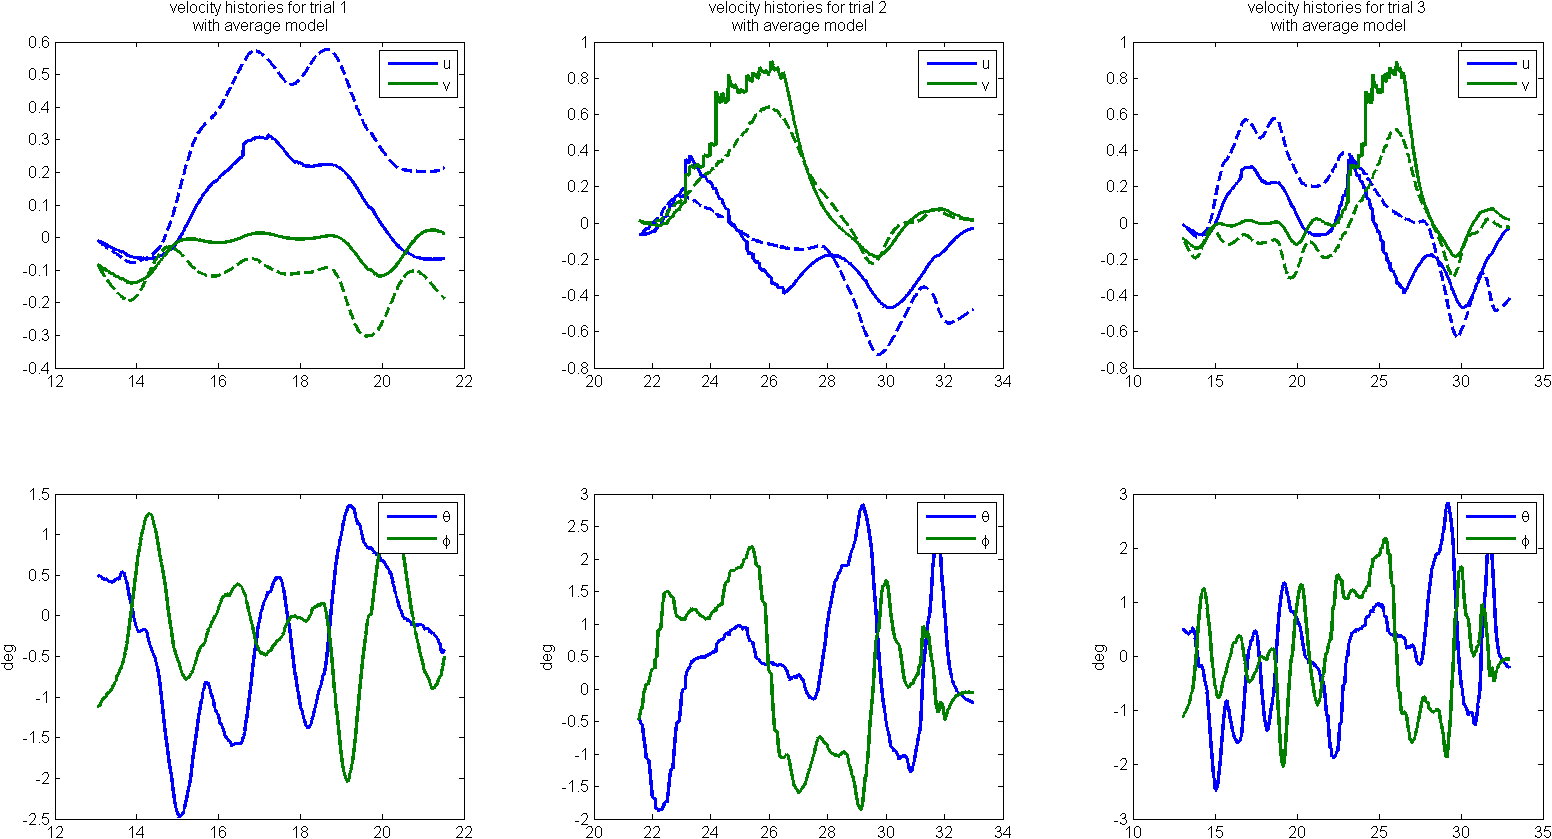
\includegraphics[width = \textwidth]{model_day_1.png}
\caption{Plots of measured outputs (solid lines) and model-predicted outputs (dashed lines) for day 1 data. Upper charts show state (velocity) histories; lower charts show measured attitude for reference.}
\label{fig:day1mse}
\end{figure}

\begin{figure}[tb!]
\centering
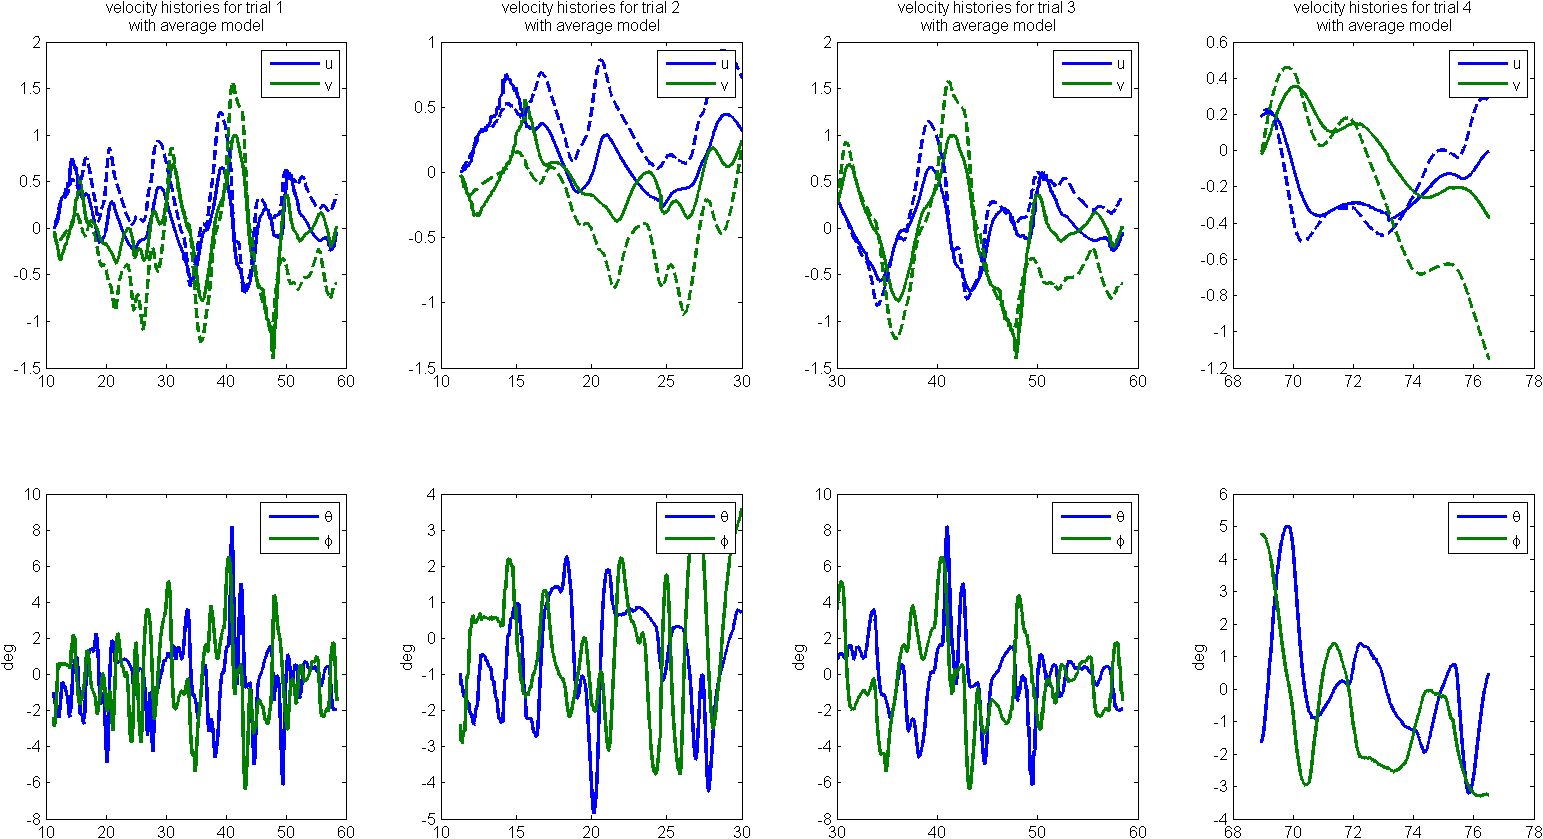
\includegraphics[width = \textwidth]{model_day_2.png}
\caption{Plots of measured outputs (solid lines) and model-predicted outputs (dashed lines) for day 2 data. Upper charts show state (velocity) histories; lower charts show measured attitude for reference.}
\label{fig:day2mse}
\end{figure}

\end{document}